\documentclass[12pt,openright,twoside,a4paper]{abntex2}
\usepackage[utf8]{inputenc}
\usepackage{times}
\usepackage[T1]{fontenc}
\usepackage{microtype}
\usepackage{amsmath,graphicx,float,amssymb,import,tikz,booktabs,mathtools,indentfirst, gensymb, adjustbox}
\usepackage[brazil]{babel}
\usepackage[style=abnt,
backref=true,
backend=biber,
citecounter=false,
backrefstyle=three,
url=false,
maxbibnames=99,
mincitenames=1,
maxcitenames=2,
backref=true,
hyperref=true,
uniquename=false,
uniquelist=false]{biblatex}
\usepackage{csquotes}
\addbibresource{Referencias.bib}
\setlength{\parindent}{1.3cm}
\setlength{\parskip}{0.2cm}
\frenchspacing
\graphicspath{{Imagens/}}
\hypersetup{
    colorlinks=false,
    linkcolor=black,
    filecolor=black,
    urlcolor=black,
    }
\titulo{\textbf{EXPERIMENTO 1: Estudo do perfil de temperatura em aletas, superfícies estendidas }}
\autor{Henrique Cândido da Silva Ramos, Isadora pires Gomes, Juan Felipe Cardoso Elias, Marco Túlio Mello Silva, Maria Letícia Teodoro Reis, Vinícius Rocha João Pinheiro}
\local{Lorena, SP}
\data{2023}
\instituicao{
Universidade de São Paulo - USP
\par
Escola de Engenharia de Lorena}
\tipotrabalho{Relatório técnico}
\preambulo{Disciplina: Laboratório de Engenharia Química II - LOQ4061 \\
Turma: 20232D1 \\
Prof. Geronimo Virginio Tagliaferro}
\begin{document}
\selectlanguage{brazil}
\imprimircapa

\imprimirfolhaderosto*

\begin{resumo}
	Tal x e y
\end{resumo}

\begin{simbolos}

	\item $\zeta$
	
	
	
	
\end{simbolos}



\tableofcontents


\textual



\chapter{Introdução}\label{ch: Introdução}
O estudo do comportamento térmico de superfícies estendidas, como aletas, desempenha um papel fundamental na análise e otimização de sistemas de transferência de calor. As aletas são estruturas projetadas para aumentar a taxa de transferência de calor entre um fluido e o ambiente circundante, sendo amplamente aplicadas em diversos setores da engenharia, como na refrigeração de equipamentos eletrônicos, trocadores de calor e sistemas de resfriamento industrial \cite{incropera2008}. %To Do arrumar o bibitex
O perfil de temperatura em aletas é um fator crítico para entender a eficiência da dissipação de calor e a distribuição de temperaturas ao longo da superfície. A compreensão detalhada das variações de temperatura nessas estruturas é essencial para projetar aletas que maximizem a transferência de calor, minimizando as perdas energéticas e otimizando o desempenho térmico dos sistemas \cite{incropera2008}.
O presente relatório tem como objetivo avaliar o perfil de temperatura de aletas em aquecimento em função do tempo. As medições foram realizadas por um termômetro digital.
Serão consideradas as seguintes variáveis nas aletas: diâmetro da aleta e propriedades do material. Além disso, serão discutidas as técnicas experimentais e numéricas empregadas para investigar o comportamento térmico das aletas e avaliar o impacto de diferentes variáveis.
Ao compreendermos o perfil de temperatura em aletas, poderemos desenvolver soluções mais eficientes e sustentáveis para o controle térmico em uma ampla gama de aplicações.



\chapter{Objetivos}\label{ch: Objetivos}



\chapter{Materiais e Métodos}\label{ch: Materiais e Métodos}

Em primeiro lugar, foi analisado quais materiais constituíam as superfícies estendidas que seriam estudadas, a A era feita de alumínio e B e C de aço (Figura \ref{fig:Figura1}).

Posteriormente, utilizou-se o paquímetro para medir o diâmetro das aletas (Figura \ref{fig:Figura2}) sendo elas 9.5 $mm$, 15 $mm$ 15 $mm$, respectivamente.
\begin{figure}[H]
	\caption{Aletas A, B e C}
	\centering
	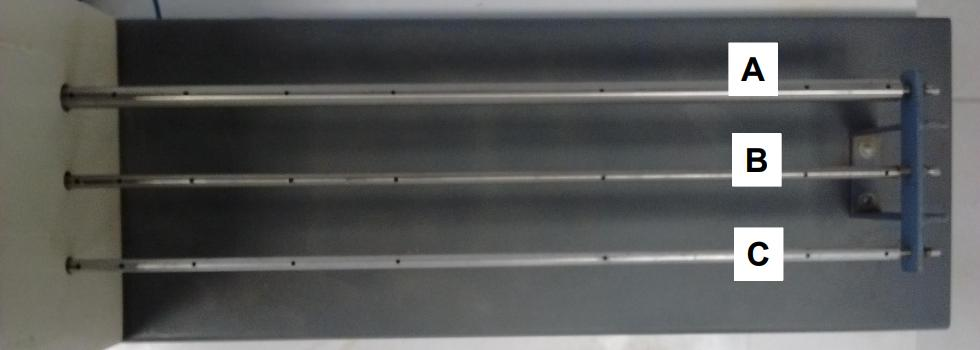
\includegraphics[scale=0.4]{figura1.jpg}
	\legend{Fonte: Tagliaferro (2021)}
	\label{fig:Figura1}
\end{figure}

\begin{figure}[H]
	\caption{Medição do diâmetro da aleta}
	\centering
	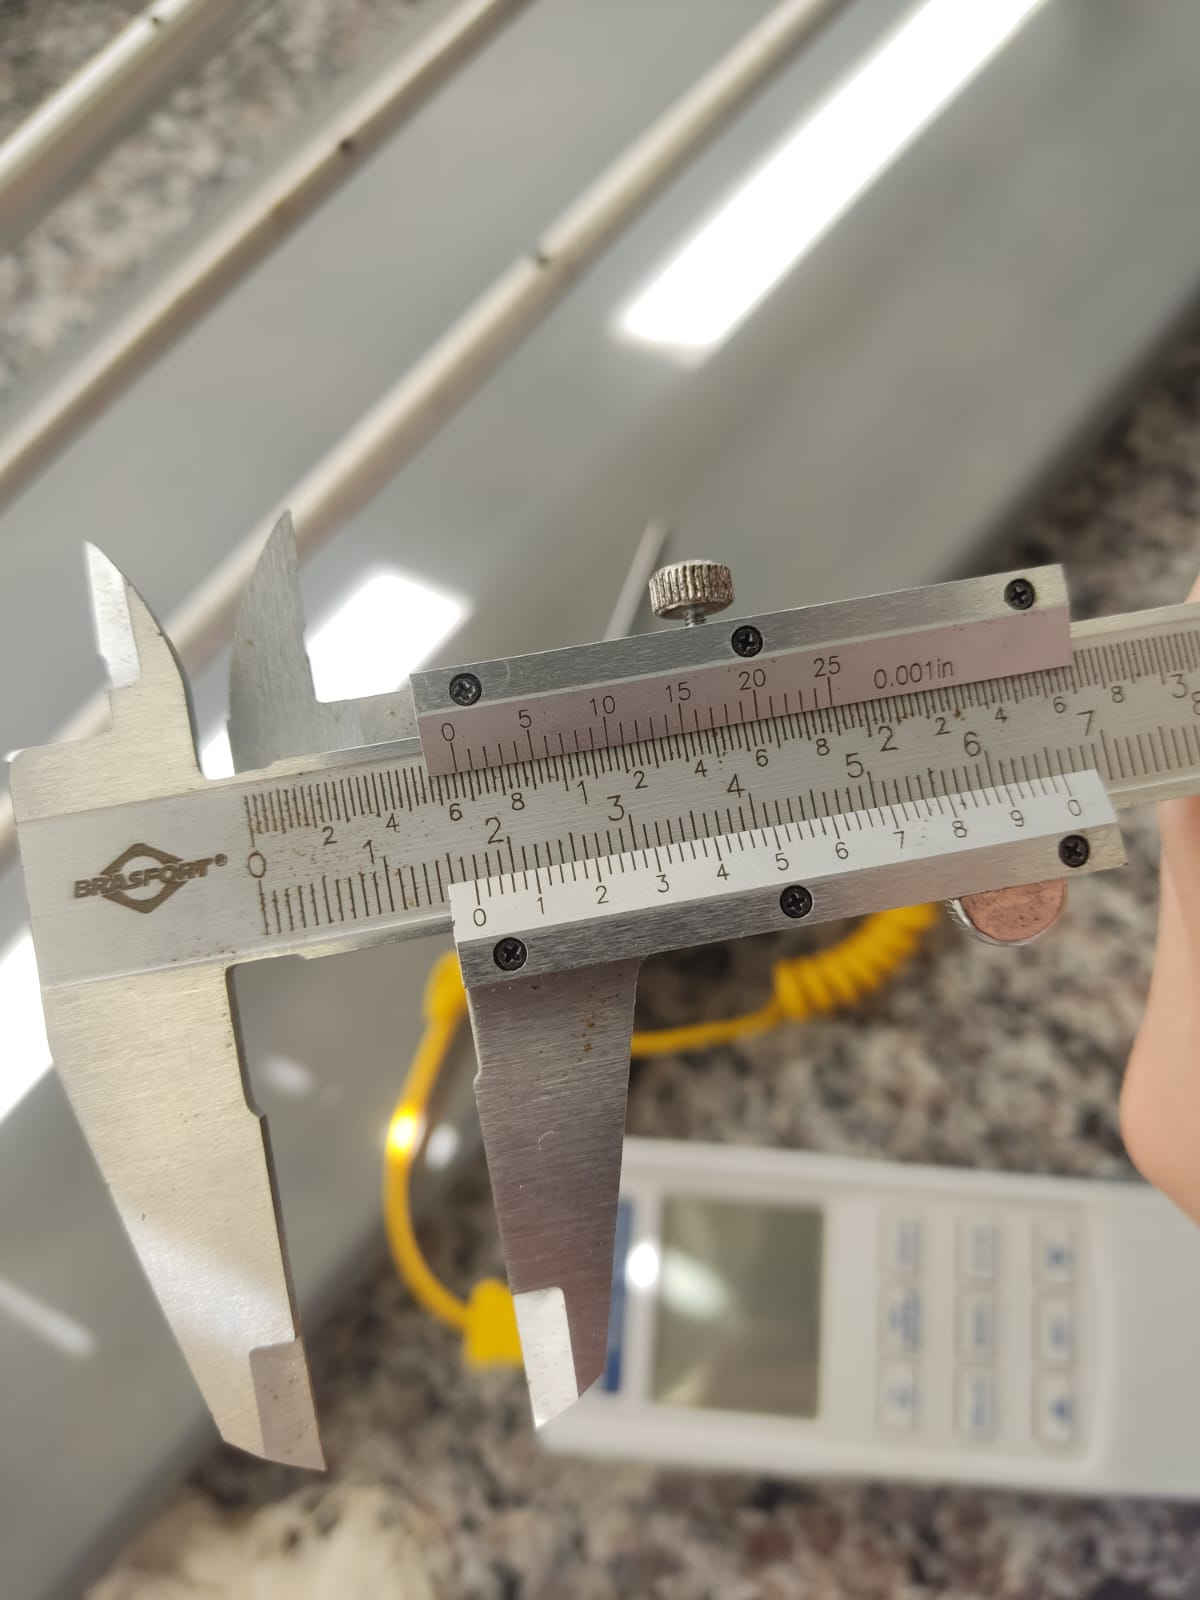
\includegraphics[scale=0.15]{figura2.jpg}
	\legend{Fonte: Autores}
	\label{fig:Figura2}
\end{figure}

Com o auxílio de uma régua, foi possível medir a distância de cada ponto de coleta de temperatura - a temperatura foi medida a partir do termômetro (Figura \ref{fig:Figura3}). O equipamento utilizado no experimento (Figura \ref{fig:Figura4}) continha as aletas estendidas conectadas ao banho termostático que transmitia calor para as mesmas. Para medir o tempo de cada intervalo de medição, utilizou-se três cronômetros para que assim a medição fosse mais fidedigna (Figura \ref{fig:Figura5}).





\begin{figure}[H]
	\caption{Medição da temperatura}
	\centering
	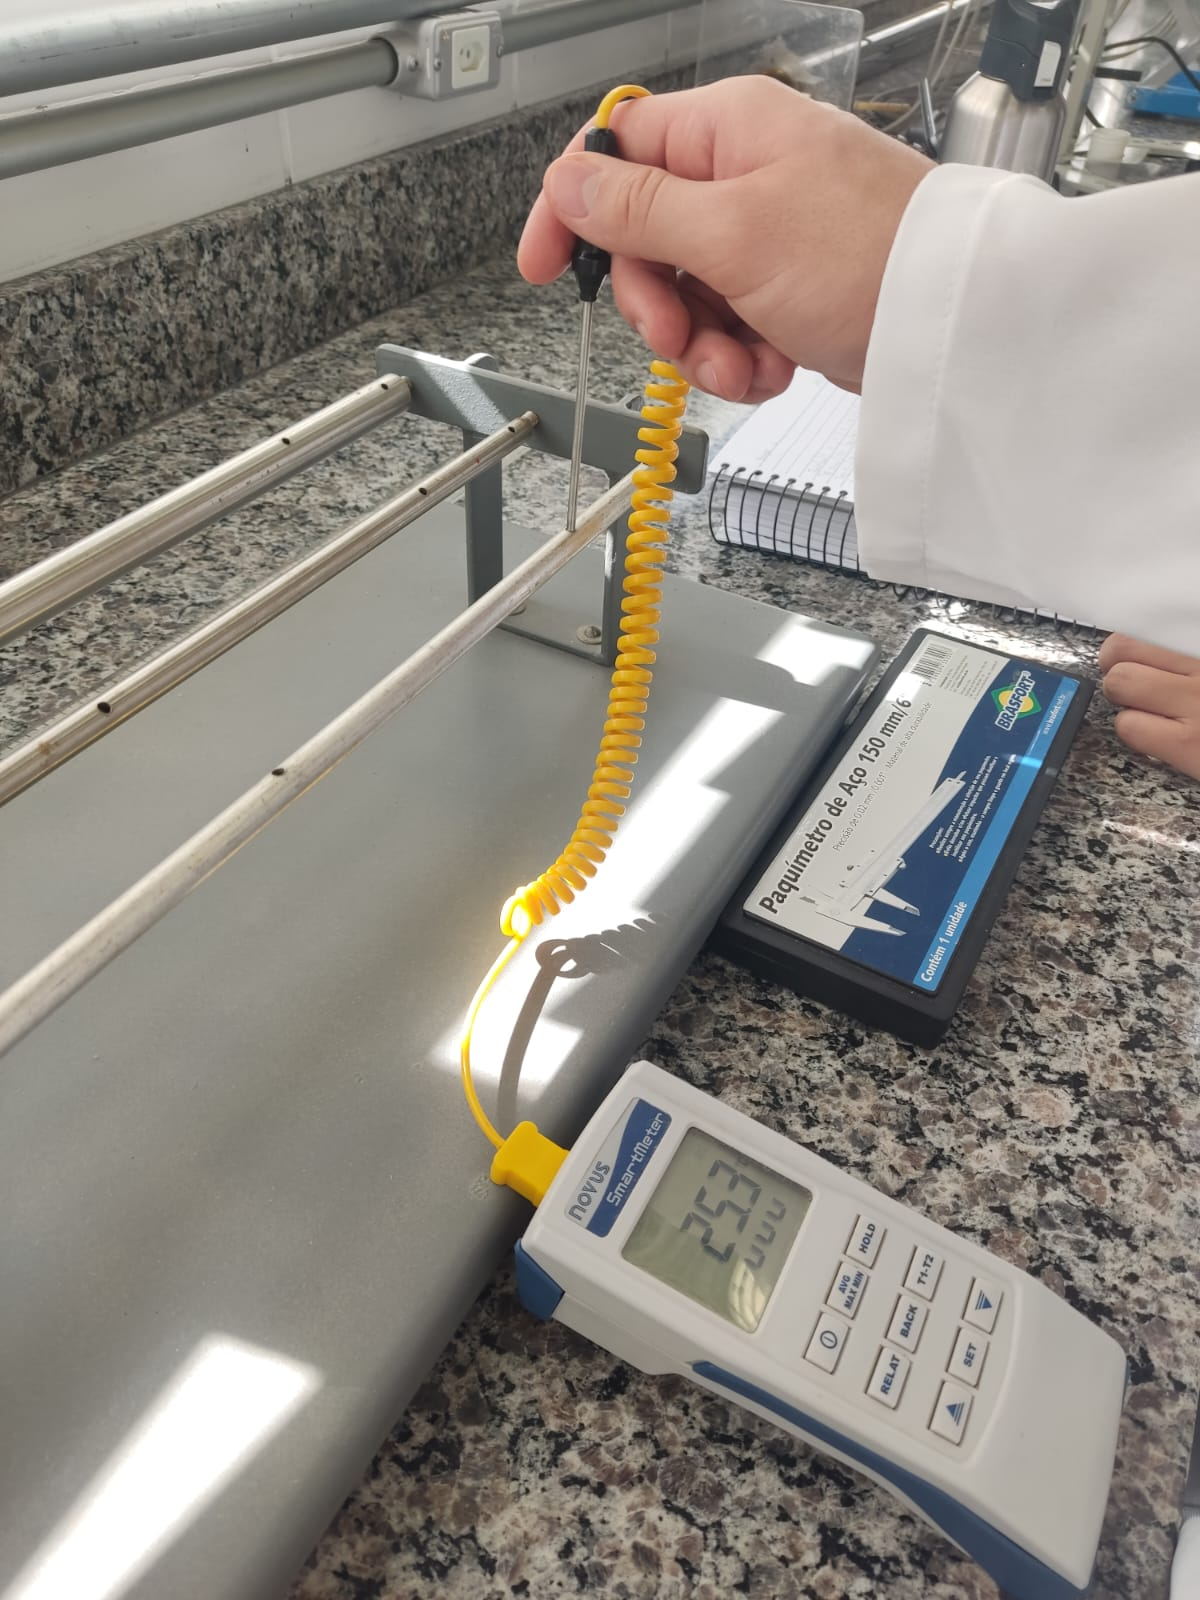
\includegraphics[scale=0.2]{figura3.jpg}
	\legend{Fonte: Autores}
	\label{fig:Figura3}
\end{figure}

\begin{figure}[H]
	\caption{Equipamento utilizado no experimento}
	\centering
	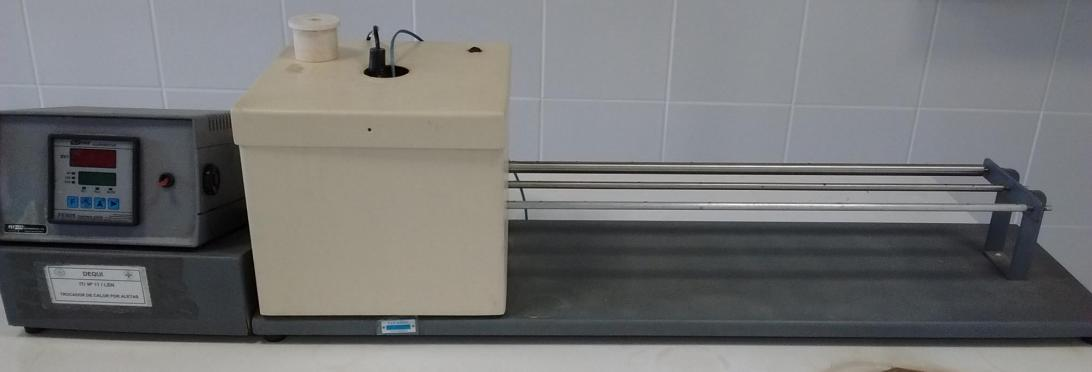
\includegraphics[width=0.75\textwidth]{figura4.jpg}
	\legend{Fonte: Autores}
	\label{fig:Figura4}
\end{figure}

\begin{figure}[H]
	\caption{utilização dos Cronômetros}
	\centering
	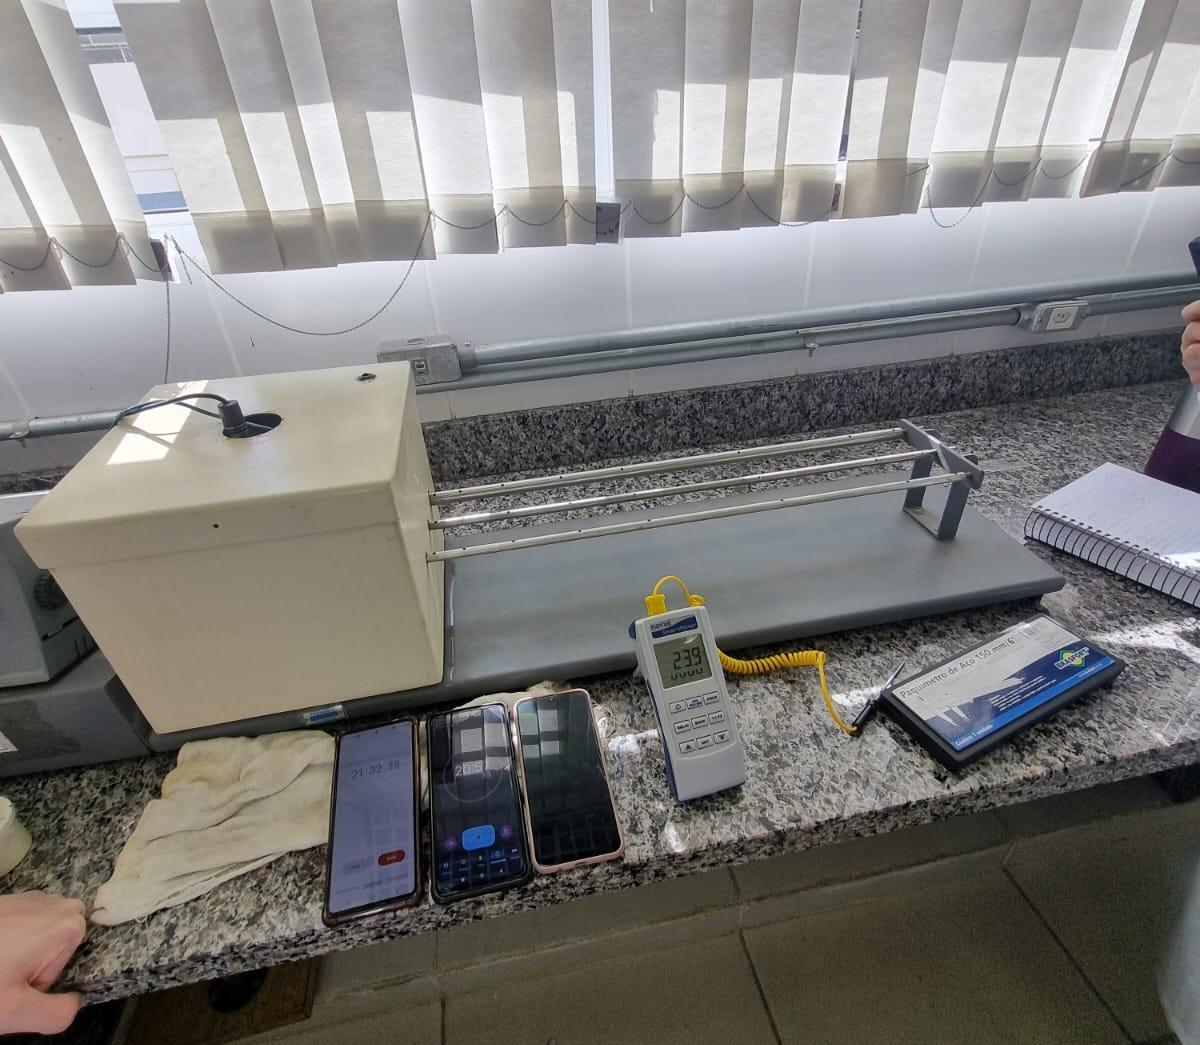
\includegraphics[width=0.75\textwidth]{figura5.jpg}
	\legend{Fonte: Autores}
	\label{fig:Figura5}
\end{figure}

Utilizando um termômetro, foi medida a temperatura inicial das aletas na posição 8 cm. Em seguida, avaliou-se a temperatura nessa posição a cada 4 minutos, para verificar o perfil de temperatura e se estão sob regime permanente de transferência de calor. Posteriormente, estimou-se a temperatura ambiente e, consequentemente, analisou-se outras posições das aletas para ver como se comportavam em relação à distância do ponto inicial, onde o banho termostático dissipava calor para o restante da superfície estendida. Através desses dados, determinou-se o coeficiente de convecção, taxa de transferência e eficiência de cada aleta, considerando a relação entre o material e o diâmetro de cada uma delas.

\chapter{Resultados}\label{ch: Resultados}
Como primeiro passo, foi determinado a condição de contorno que seria aplicada no experimento. Foi determinado que o diâmetro de todas as aletas são mais do que 20 vezes menores que o comprimento, logo a condição de contorno aplicável é a de aleta infinita.
\begin{align}
	\label{eq:dem cond_contorno}
	\frac{\text{Diâmetro}}{\text{Comprimento}} & \geq 20                              \\
	\frac{9.5 \cdot 10^{-3}}{60 \cdot 10^{-2}} & > 20  \implies \text{Aleta infinita} \\
	\frac{15 \cdot 10^{-3}}{60 \cdot 10 ^{-2}} & > 20 \implies \text{Aleta infinita}
\end{align}
Portanto, as condições de contorno para o experimento são as seguintes:
\begin{align}
	\label{eq:cond_contorno}
	\theta(0) & = T_0 \\
	\theta(L) & = 0
\end{align}
Para os cálculos foram utilizadas as seguintes equações:

\begin{equation}
	\label{eq:theta theta_0}
	\frac{\theta(x)}{\theta_0} = \exp \left( - \frac{hP}{kA}x \right)
\end{equation}
Onde \(\frac{\theta(x)}{\theta_0}\) é a temperatura admensionalizada, que é dada por

\begin{equation}
	\label{eq:temp admens}
	\frac{\theta(x)}{\theta_0} = \frac{T(x) - T_{\infty}}{T_0 - T_{\infty}}
\end{equation}
Onde \(T\) é a temperatura da aleta em um ponto qualquer, \(T_{\infty}\) é a temperatura ambiente, \(T_0\) é a temperatura na base da aleta.
Como a aleta é uma em formato de pino, podemos simplificar o expoente da equação \eqref{eq:theta theta_0} para, pois \(P = 2 \pi r\), onde \(r\) é o raio da aleta, e \(A = \pi r^2\), então

\begin{equation}
	\label{eq:expoente}
	\frac{hP}{kA_{tr}} = \frac{2h}{k \cdot r}
\end{equation}
Onde \(r\) é o raio da aleta.

Para o cálculo da taxa de transferência de calor, utilizou-se a seguinte equação:

\begin{align}
	\label{eq:taxa de transferencia}
	M & = -k A_{Tr} \frac{\mathrm{d}\theta}{\mathrm{d}x} \bigg|_{x=0} \\
	  & = \int_{0}^{\infty} h P \theta \mathrm{d}x                    \\
	M & = \sqrt{hPA_{Tr}k} \theta_b
\end{align}

Onde \(M\) é a taxa de transferência de calor, \(k\) é a condutividade térmica do material, \(A_{Tr}\) é a área de transversal, \(h\) é o coeficiente de convecção, \(\theta\) é a temperatura admensionalizada, \(P\) é o perímetro da aleta e \(\theta_b\) é a temperatura na base da aleta.

Para a eficiência da aleta, utilizou-se a seguinte equação:

\begin{equation}
	\label{eq:eficiencia}
	\eta = \frac{1}{L} \cdot \frac{1}{\sqrt{\frac{2h}{k \cdot r}}}
\end{equation}

% TODO Arrumar essa equação acima
Os valores de condutividade térmica do alumínio e do aço foram retirados da tabela 1.1 do livro de Incropera \cite{incropera2008}, e são respectivamente 237 \(\frac{W}{m} \cdot K\) e 71 \(\frac{W}{m} \cdot K\). Os perímetros das aletas de diâmetro de 9.5 \(mm\) valem

\begin{align}
	P & = \pi \cdot 9.5 \cdot 10^{-3} \\
	  & = 2.984 \cdot 10^{-2}
\end{align}

Já para a aleta de 15 \(mm\) temos

\begin{align}
	P & = \pi \cdot 15 \cdot 10 {^-3} \\
	  & = 4.712 \cdot 10{-2}
\end{align}

A área de seção transversal para as aletas de 9.5 \(mm\) valem

\begin{align}
	A & = \pi \left( \frac{D}{2} \right)^2                 \\
	  & = \pi \left( \frac{9.5 \cdot 10^{-3}}{2} \right)^2 \\
	  & = 7.088 \cdot10 ^{-5} \; m^2
\end{align}

Para a aleta de 15  \(mm\)  a área fica

\begin{equation}
	A = \pi \left( \frac{15 \cdot 10^{-3}}{2} \right)^2 = 1.7671 \cdot 10^{-4} \; m^2
\end{equation}
Os dados coletados são apresentados a seguir

\begin{table}[H]
	\centering
	\caption{Temperatura em função do tempo}
	\begin{adjustbox}{width=0.95\textwidth,center=\textwidth}
		\begin{tabular}{c|c|c|c|c|c|c|c|c}
			\toprule
			Tempo (min) & 0                  & 4                  & 8                  & 12                 & 16                 & 20                  & 24                  & 28                 \\
			\midrule
			Aleta A     & 28.2 \(\degree C\) & 28.7 \(\degree C\) & 28.7 \(\degree C\) & 28.4 \(\degree C\) & 29.3 \(\degree C\) & 29.16 \(\degree C\) & 29.8 \(\degree  C\) & 29.9\(\degree C\)  \\
			Aleta B     & 24.1 \(\degree C\) & 24.7 \(\degree C\) & 24.8 \(\degree C\) & 25.5 \(\degree C\) & 25.5 \(\degree C\) & 26.1 \(\degree C\)  & 26.2 \(\degree  C\) & 28.2\(\degree C\)  \\
			Aleta C     & 37.4 \(\degree C\) & 39.3 \(\degree C\) & 38.7 \(\degree C\) & 39.1 \(\degree C\) & 38.4 \(\degree C\) & 38.5 \(\degree  C\) & 39.1 \(\degree  C\) & 38.8 \(\degree C\) \\
			
			\bottomrule
		\end{tabular}
	\end{adjustbox}
	\legend{Fonte: Autores}
	\label{tab:temp_tempo}
\end{table}

\begin{table}[H]
	\centering
	\caption{Temperatura em Função da Posição}
	\begin{adjustbox}{width=0.95\textwidth,center=\textwidth}
		\begin{tabular}{c|c|c|c|c|c|c|c|c}
			\toprule
			x \((cm)\) & 0                   & 3                   & 8                   & 15                 & 22.5                & 37.5                & 52.5                & 60                  \\
			\midrule
			Aleta A    & 44.3 \(\degree C\)  & 38.2 \(\degree C\)  & 30.9 \(\degree C\)  & 26.0 \(\degree C\) & 23.9 \(\degree C\)  & 22.1 \(\degree  C\) & 22.6 \(\degree  C\) & 22.8 \(\degree  C\) \\
			Aleta B    & 36.8 \(\degree C\)  & 32.7 \(\degree C\)  & 28.2 \(\degree C\)  & 25.2 \(\degree C\) & 23.6 \(\degree C\)  & 23.6 \(\degree  C\) & 23.6 \(\degree  C\) & 23.6 \(\degree  C\) \\
			Aleta C    & 47.5 \(\degree  C\) & 44.2 \(\degree  C\) & 39.6 \(\degree  C\) & 34.6 \(\degree C\) & 30.9 \(\degree  C\) & 26.5 \(\degree C\)  & 24.4 \(\degree C\)  & 24.3 \(\degree C\)  \\
			\bottomrule
		\end{tabular}
	\end{adjustbox}
	\legend{Fonte: Autores}
	\label{tab:temp_posicao}
\end{table}

É importante notar que na tabela \ref{tab:temp_posicao}, em principal na aleta C, teve ocorrência da interferência do sol que estava irradiando sobre as partes finais da mesma, fazendo com que sua temperatura saísse do padrão esperado.

\section{Determinação do coeficiente de convecção para as aletas} % (fold)
\label{sec:determinacao_h}
Para o calculo da determinação do coeficiente convectivo, utilizou-se da equação \eqref{eq:theta theta_0}. Como é necessário um ponto com temperatura conhecida, utilizou-se o ponto que dista \(0.3 \; cm\) da base da aleta, para os cálculos. A temperatura da base é o primeiro ponto, que dista  \(0 \; cm\) e a temperatura ambiente considerada foi de  \(21.5 \degree \; C\). Isolando nossa equação em função de  \(h\) temos

\begin{equation}
	h = \left( \ln \frac{\theta_0}{\theta} \right)^2 \cdot \frac{k \cdot r}{2 \cdot x}
\end{equation}
Os valores encontrados são apresentados abaixo

\begin{table}[H]
	\caption{Valores coeficiente convectivo}
	\centering
	\begin{tabular}{c|c|c|c}
		\toprule
		Aleta                                       & A       & B       & C      \\
		\midrule
		h \(\left[ \frac{W}{m^2 \cdot K} \right] \) & 28.6781 & 18.2313 & 11.755 \\
		\bottomrule
	\end{tabular}
	\legend{Fonte:Autores}
	\label{tab:valores_h}
\end{table}
% section  (end)
%

\section{Distribuição Teórica versus Real}

Foram realizados as curvas das distribuições de temperatura teórica, utilizando os valores de h calculados em \ref{sec:determinacao_h}. Aplicando novamente na equação \eqref{eq:theta theta_0}, substituindo os valores e isolando para a temperatura, a equação da curva fica

\begin{equation}
	T = (T_B - T_{\infty}) \exp\left(- \sqrt{\frac{2h}{k\cdot r}}\cdot x\right) + T_\infty
\end{equation}
Onde os devidos valores foram substituídos para cada aleta. Os gráficos são apresentados a seguir
% --TODO Arrumar esse gráfico que ta trocado
\begin{figure}[H]
	\caption{Distribuição Real x Teórica}
	\begin{center}
		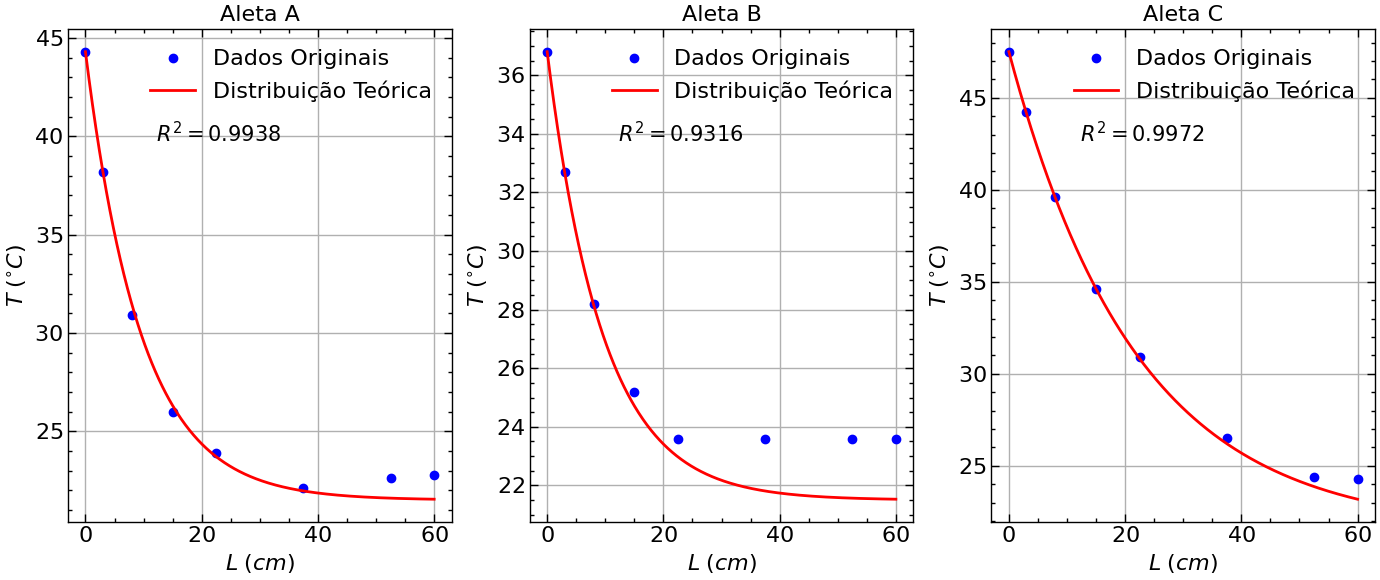
\includegraphics[width=0.95\textwidth]{Imagens/distribuicoes.png}
	\end{center}
	\legend{Fonte: Autores}\label{fig:real_x_teorica}
\end{figure}

\section{Taxa de transferência de calor}

A taxa de transferência de calor foi calculada utilizando a fórmula \eqref{eq:taxa de transferencia}, onde para os valores de \(\theta_0\) valem, para as aletas A, B e C respectivamente \(\theta_{0,A} = 22.8 \degree C\), \(\theta_{0, B} = 15.3 \degree C\) e \(\theta_{0,C} = 26 \degree C\). A taxa de calor é mostrada abaixo

\begin{table}[H]
	\caption{Taxa de transferência}
	\centering
	\begin{tabular}{c|c|c|c}
		\toprule
		Aleta                   & A      & B      & C      \\
		\midrule
		M \(\left[ W \right] \) & 2.9687 & 0.8005 & 1.9958 \\
		\bottomrule
	\end{tabular}
	\legend{Fonte:Autores}
	\label{tab:valores_troca}
\end{table}

\section{Eficiência de cada Aleta}

A eficiência de cada aleta foi calculada pela fórmula \eqref{eq:eficiencia}. Os resultados são apresentados abaixo

\begin{table}[H]
	\caption{Eficiência de cada Aleta}
	\centering
	\begin{tabular}{c|c|c|c}
		\toprule
		Aleta    & A       & B       & C      \\
		\midrule
		\(\eta\) & 0.16059 & 0.16029 & 0.3655 \\
		\bottomrule
	\end{tabular}
	\legend{Fonte:Autores}
	\label{tab:eficiencia}
\end{table}

\section{Ultima Conta, não sei oq é}

\chapter{Conclusão}\label{ch: conclusões}



\printbibliography[title={Referências}]
\end{document}

